%!TEX root = ../main.tex
\section{Field Dataset}\label{sec:field-dataset}

% \begin{figure}[htbp]
%   \centering
%   \includegraphics[width=0.70\textwidth]{figure/60_data/}
%   \caption{
%     }
%     \label{fig:}
% \end{figure}

\begin{figure}[htbp]
  \centering % 図全体を中央揃え

  % 1つ目の画像(幅を1.0にして縦積みを強制し、中央揃えにする)
  \begin{subfigure}[b]{1.0\linewidth}
    \centering
    \includegraphics[height=8cm, keepaspectratio]{figure/60_data/study_area.png}
    \caption{宇治市の概要。}
    \label{fig:japan-and-uji-city}
  \end{subfigure}

  \vspace{1em} % 画像間のスペース

  % 2つ目の画像
  \begin{subfigure}[b]{1.0\linewidth}
    \centering
    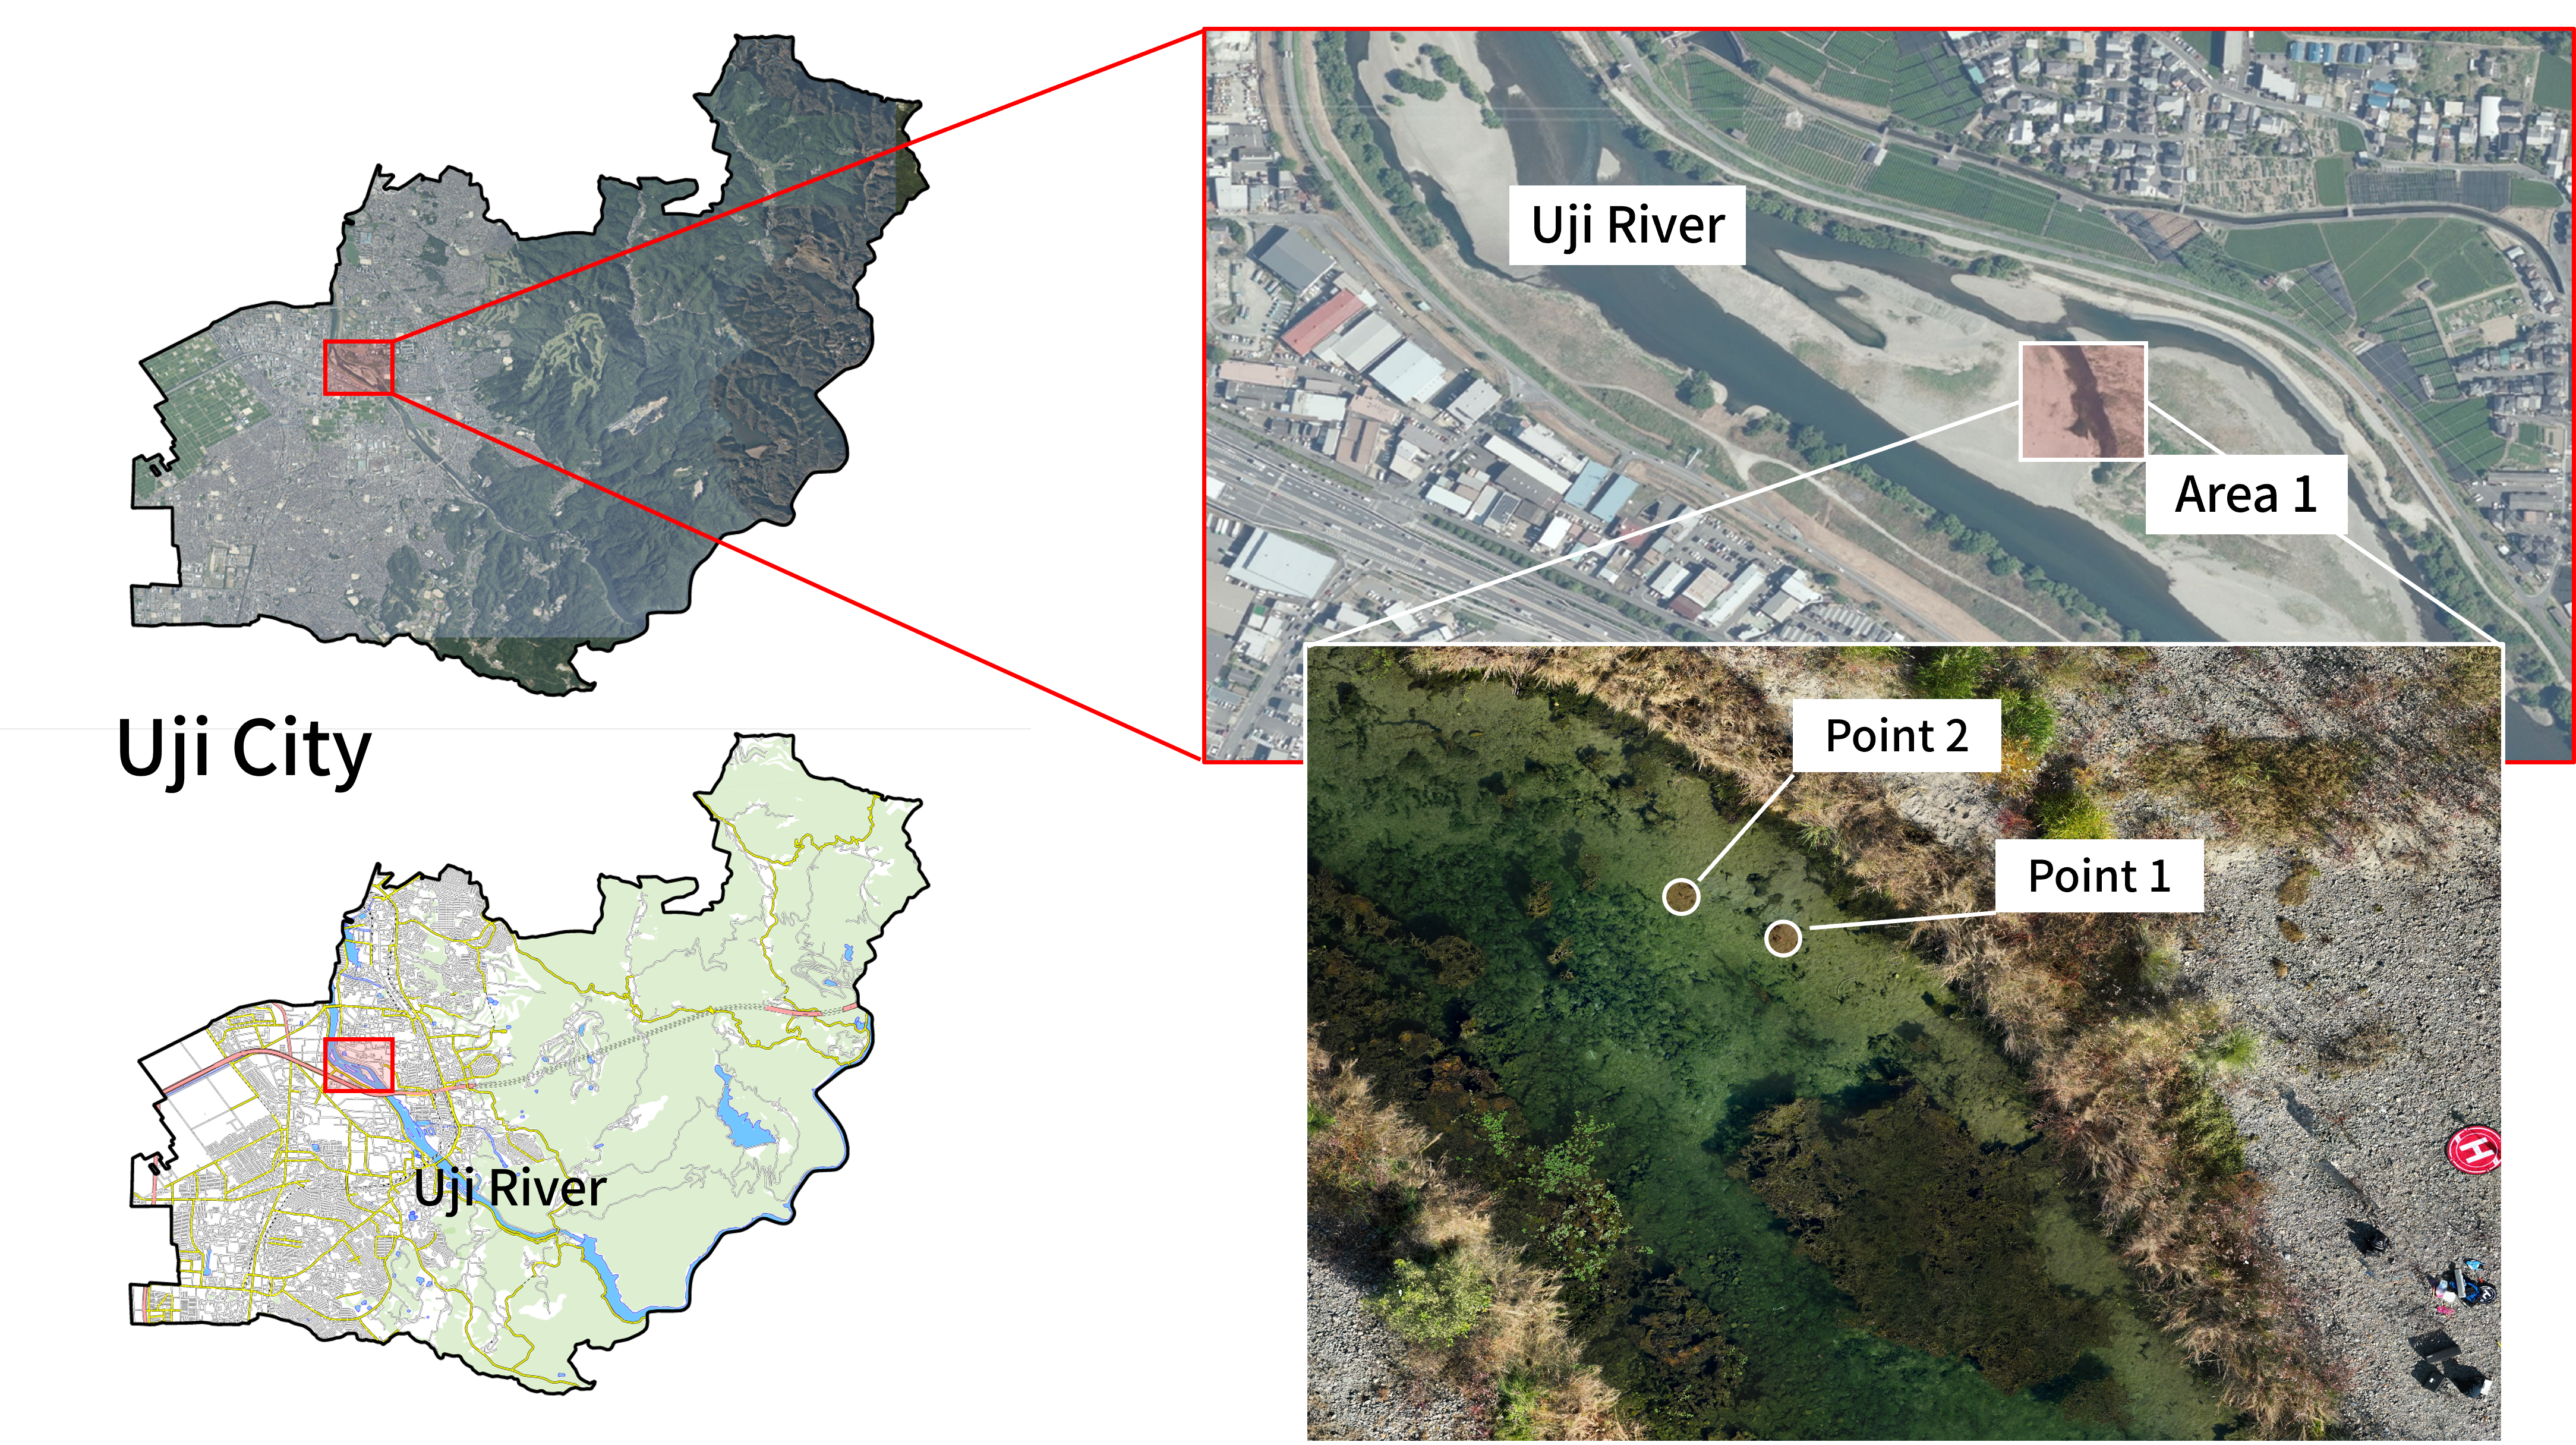
\includegraphics[height=10cm, keepaspectratio]{figure/60_data/area1.png}
    \caption{調査地域の概要。}
    \label{fig:area1_map}
  \end{subfigure}

  % 全体のキャプション
  \caption{
    調査対象地域の概要図。
    対象は、日本の京都府に位置する宇治市街を流れる宇治川の中流域である。
    本流から分派し水が滞留している箇所を対象にUAVから撮影を行った。
    広域航空写真は国土地理院~\cite{gsi_aerial_photo}、地図はOpen Street Map~\cite{OpenStreetMap}を使用した。
  }
  \label{fig:study-area}
\end{figure}

\missingfigure{scale Bar入れるの忘れてた!!}

\subsection{Study Area}\label{subsec:study-area}



% \begin{figure}[htbp]
%   \centering
%   \includegraphics[width=0.70\textwidth]{figure/60_data/study_area_overview.png}
%   \caption{調査対象地域の概要図。京都府宇治市の宇治川中流域でUAV調査を行った。}
%   \label{fig:study-area}
% \end{figure}

実世界における手法の検証には、京都府宇治市を流れる宇治川中流域にて取得したデータセット(Real-world data)を使用した。
データの取得は2025年11月15日の午前9:00から10:30にかけてArea1を対象に実施した
%(\cref{fig:study-area})
。
% データの取得は2025年11月15日の午前9:00から10:30にかけて実施し、同水域内の異なる2箇所(Area 1, Area 3)を対象とした。
\note{まだArea3を使用するか決めていない。2が環境が異なる(大きな礫が多い河床)だが、RTK情報がないため厳しい。3は試したいが、影とそれ以外の輝度差の大きい条件}
撮影時の気象条件は晴れであり、Area 1観測時における気温は12.8$^\circ$Cから16.3$^\circ$C、風速は0.5から0.9 m/sと極めて穏やかで、UAVおよび光学センサーによる水域観測に最適な環境であった。
% \url{https://www.data.jma.go.jp/stats/etrn/view/10min_s1.php?prec_no=61&block_no=47759&year=2025&month=11&day=15&view=}
本調査では、流速が速い本流ではなく、流れから分派し水が滞留している副次的な水路(Second channel)を対象とした。
この水域は波が穏やかで透明度が極めて高い。

% \subsubsection{Area 1}\label{subsec:area-1}
目視による推定最大水深は約1.5mであり、水面の一部には浮遊植物が確認された。
また、河床には藻類が生育しており、これにより水底が均質な砂礫ではなく視覚的に豊富なテクスチャを有している。
これは後述する画像からの三次元再構成を有利にする条件である。
取得されたUAV画像の特徴的な例は、%\cref{fig:field-data}%
に示す。

% \begin{figure}[htbp]
%   \centering
%   \includegraphics[width=0.70\textwidth]{figure/60_data/}
%   \caption{
%     各AreaのUAV画像の特徴的な例。
%     }
%     \label{fig:field-data}
% \end{figure}


% \note{
%   * ここでは、撮影エリアでの特徴に終始するぞ。
%   * 水面には水草が浮いているぞ。
%   * 本流ではなく、水たまりになっているSecond Channelにおいて撮影したぞ。
%   * 最大深度は1.5mほどだと推定されるぞ。
%   * Textureも比較的豊富だぞ。
%   * 透明度が高く、波も穏やかだぞ。
%   * 気温や湿度、天気はこの程度だった。(撮影時14度、湿度60\%、快晴)(後に正確に調べ直す)
% }


\subsection{UAV Platform}\label{subsec:uav-platform}


\begin{figure}[htbp]
  \centering

  \begin{minipage}[t]{0.45\linewidth}
    \centering
    \includegraphics[height=4cm, keepaspectratio]{figure/60_data/mavic3e.png}
    \caption{DJI Mavic 3 Enterprise}
    \label{fig:mavic3e}
  \end{minipage}
  % \hspace{0.5cm}
  \hfill
  \begin{minipage}[t]{0.45\linewidth}
    \centering
    \includegraphics[height=4cm, keepaspectratio]{figure/60_data/area1_riverbed-from-ground.JPG}
    \caption{地上から撮影したArea 1の河床。水面には浮遊植物、河床には藻類が生育している。}
    \label{fig:area1_riverbed-from-ground}
  \end{minipage}

  % \caption{#8}
  % \label{#9}
\end{figure}

画像の取得には、RTK-GPS(Real-Time Kinematic Global Positioning System)を搭載したUAV(Unmanned Aerial Vehicle)プラットフォームを使用した。
RTK測位を用いることで、センチメートル級の高精度な位置情報が各画像に付与されるため、地上基準点(GCP: Ground Control Points)を現地に設置することなく、高精度なSfM(Structure from Motion)処理が可能となっている。
\checkref{根拠となる論文を引っ張ってくる}

また、本研究では水底の三次元形状およびテクスチャを鮮明に捉えることを最優先としたため、カメラレンズに円偏光(Circular Polarized Light :CPL)フィルターを装着した。
これにより、水面における太陽光の反射(Sun Glint)を物理的に抑制している。
偏光フィルターの使用は取得画像の放射輝度値(Radiance)に影響を与え、厳密なラジオメトリック補正の不確実性を増加させる可能性があるが、本研究の範囲においては水面反射に伴う環境光のモデル化を考慮していないため、水面下の可視性を最大化するアプローチを採用した。


画像の取得には、RTK-GPS(Real-Time Kinematic Global Positioning System)を搭載した商用UAV、DJI Mavic 3 Enterprise\cite{DJI-Mavic-3-Enterprise}を使用した。
本機体は4/3型CMOSセンサー(有効画素数20MP)を搭載し、最大5280×3956ピクセルの高解像度画像を取得可能である
(\cref{tab:drone-spec}を参照)。
レンズは35mm判換算で24mm相当(FOV: 84$^\circ$、絞り: f/2.8-f/11)の広角レンズを使用している。
撮影時は、絞りをf/2.8に固定している。
\note{被写界深度を大きくやレンズ歪みを小さくするため、ピンホールカメラに近づけるよう小さな絞り(→f/11)を使用するべきだが、Motion Blurを抑制するためにシャッタースピードを高くすることが優先のため、デフォルトで多いな口径を使用しているのか。
DroneのObliqueを含めたPath設定・ シャッタースピードの固定、含めもっとたくさん設定できることが合った。
https://gemini.google.com/app/fc2bebc9e9d48912
}
RTK測位の精度は水平方向で1cm + 1ppm、垂直方向で1.5cm + 1ppm(RMS)であり、地上基準点(GCP: Ground Control Points)を現地に設置することなく、センチメートル級の絶対位置精度を持つSfMモデルの構築が可能である。
\checkref{根拠となる論文を引っ張ってくる}
% \note{ppmは「100万分の1」という意味です。測位においては、**「基準局から1km(100万mm)離れるごとに、1mmの誤差が加算される」**ことを意味します。 つまり、基準局と移動局(ドローンやトラクターなど)の距離(ベースライン)に比例して増える誤差です。}

また、本研究では水底の三次元形状およびテクスチャを鮮明に捉えることを最優先としたため、カメラレンズに円偏光(CPL)フィルターを装着した。
これにより、水面における太陽光の反射(Sun Glint)を物理的に抑制している。
偏光フィルターの使用は取得画像の放射輝度値(Radiance)に影響を与え、厳密なRadiometic Correction(\cref{sec:color-correction})の不確実性を増加させるが、
本研究の範囲においては水面反射における環境光による反射を考慮していないため、水面下の可視性を最大化するアプローチを採用した。


\begin{table}[htbp]
  \centering
  \caption{UAVプラットフォームおよびカメラの主要諸元}
  \label{tab:drone-spec}
  \begin{tabular}{@{}ll@{}}

    \toprule
    \textbf{Category} & \textbf{Specification} \\
    
    \midrule
    \textbf{UAV Platform} & \\
    \quad Model & DJI Mavic 3 Enterprise \\
    \quad Positioning System & Onboard RTK Module \\
    
    \midrule
    \textbf{Camera Specifications} & \\
    \quad Image Sensor & 4/3 CMOS \\
    \quad Effective Pixels & 20 MP \\
    \quad Max Image Size & 5280 $\times$ 3956 pixels \\
    \quad Field of View (FOV) & 84$^\circ$ \\
    \quad Equivalent Focal Length & 24 mm \\
    \quad Aperture & f/2.8  \\ % -- f/11 だが、撮影時はf/2.8で固定?
    \quad Focus Range & 1 m to $\infty$ \\
    \quad Additional Filter & Circular Polarizing (CPL) Filter \\
    
    \midrule
    \textbf{RTK Positioning Accuracy} & \\
    \quad Horizontal (RMS) & 1 cm + 1 ppm \\
    \quad Vertical (RMS) & 1.5 cm + 1 ppm \\

    \midrule
    \textbf{Flight Mission} & \\
    \quad Flight Altitude from Water Level & 12 m \\
    \quad Nadir Images & 108 \\
    \quad Overlap Rate & 90\% \\
    \quad Side Overlap Rate & 90\% \\
    \quad Oblique Images & 80 \\
    \quad Tilt Angle & 45$^\circ$ \\

    \bottomrule
  \end{tabular}
\end{table}

\subsection{Data Acquisition}\label{subsec:data-acquisition}

\begin{table}[htbp]
  \centering
  \caption{撮影条件の詳細}
  \label{tab:flight-mission}
  \begin{tabular}{@{}ll@{}}

    \toprule
    \textbf{Flight Mission} & \\
    \midrule
    \quad Flight Altitude from Water Level & 12 m \\
    \quad \# of Nadir Images & 108 \\
    \quad Overlap Rate & 90\% \\
    \quad Side Overlap Rate & 90\% \\
    \quad \# of Oblique Images & 80 \\
    \quad Oblique Angle & 30$^\circ$ $sim$ 45$^\circ$ \\

    \bottomrule
  \end{tabular}
\end{table}

UAVによる撮影は、多視点性を確保し、画像からの三次元再構成の幾何的な推定を強めるため、直下視(Nadir)および斜め視(Oblique)の二種類のカメラアングルを組み合わせて実施した。
高度は地上高(AGL: Above Ground Level)12mという低高度で実施し、高空間分解能の画像を確保した。
ただし、後述するワークフロー(\cref{sec:workflow})ではSfM処理は最大解像度で行ったが、提案手法のRefractive-Aware Gaussian Splattingは1/4にダウンサンプリングした画像を用いた。

Nadir画像は、オーバーラップ率を90\%、サイドラップ率を90\%に設定し、自動航行により108枚取得した。
\note{OL,SL を覚えていない。リモコンから確認しないと。計算によるとだいたい90\%になる。85\%撮った気もする}

Oblique画像については、特定の一点を中心とするマニュアル操作により、カメラのオフナディア角を主に約30$^\circ$ $sim$ 45$^\circ$ (一部、60$^\circ$を含む)で、円軌道を描くように対象地点を見下ろしながら、80枚を取得した。
カメラの角度および飛行経路の詳細は、%\cref{fig:camera-path}
に定性的に示す。

\IncludeTwoImages[6cm]
{figure/60_data/area1-4_0001.JPG}
  {Nadir画像の例}
{figure/60_data/area1-6_0059.JPG}
  {Oblique画像の例}
{Area1におけるUAV画像の例}
{fig:area1}

\begin{figure}[htbp]
  \centering
  \includegraphics[width=0.80\textwidth]{figure/60_data/camera-path.png}
  \caption{
    Area1におけるカメラパスと姿勢。NadirとObliqueの2種類のカメラアングルを組み合わせて撮影した。
    }
    \label{fig:camera-path}
\end{figure}


また、推定された水深精度の定量的な評価を行うため、現地調査において水深データの取得を行った。
調査者が実際に水域に入り、代表的なポイントに検証用ターゲットを設置した上で(\cref{fig:area1_map}参照)、メジャーを用いた手動計測により水深を測定した。
測定された検証点の水深は、それぞれ61cmおよび71cmの計2点である。
地点の正確な座標は水域内であるため計測できず、検証時には、三次元復元データからターゲットを視認し、手動で座標を特定した。

\begin{figure}[htbp]
  \centering

  \begin{minipage}[t]{0.45\linewidth}
    \centering
    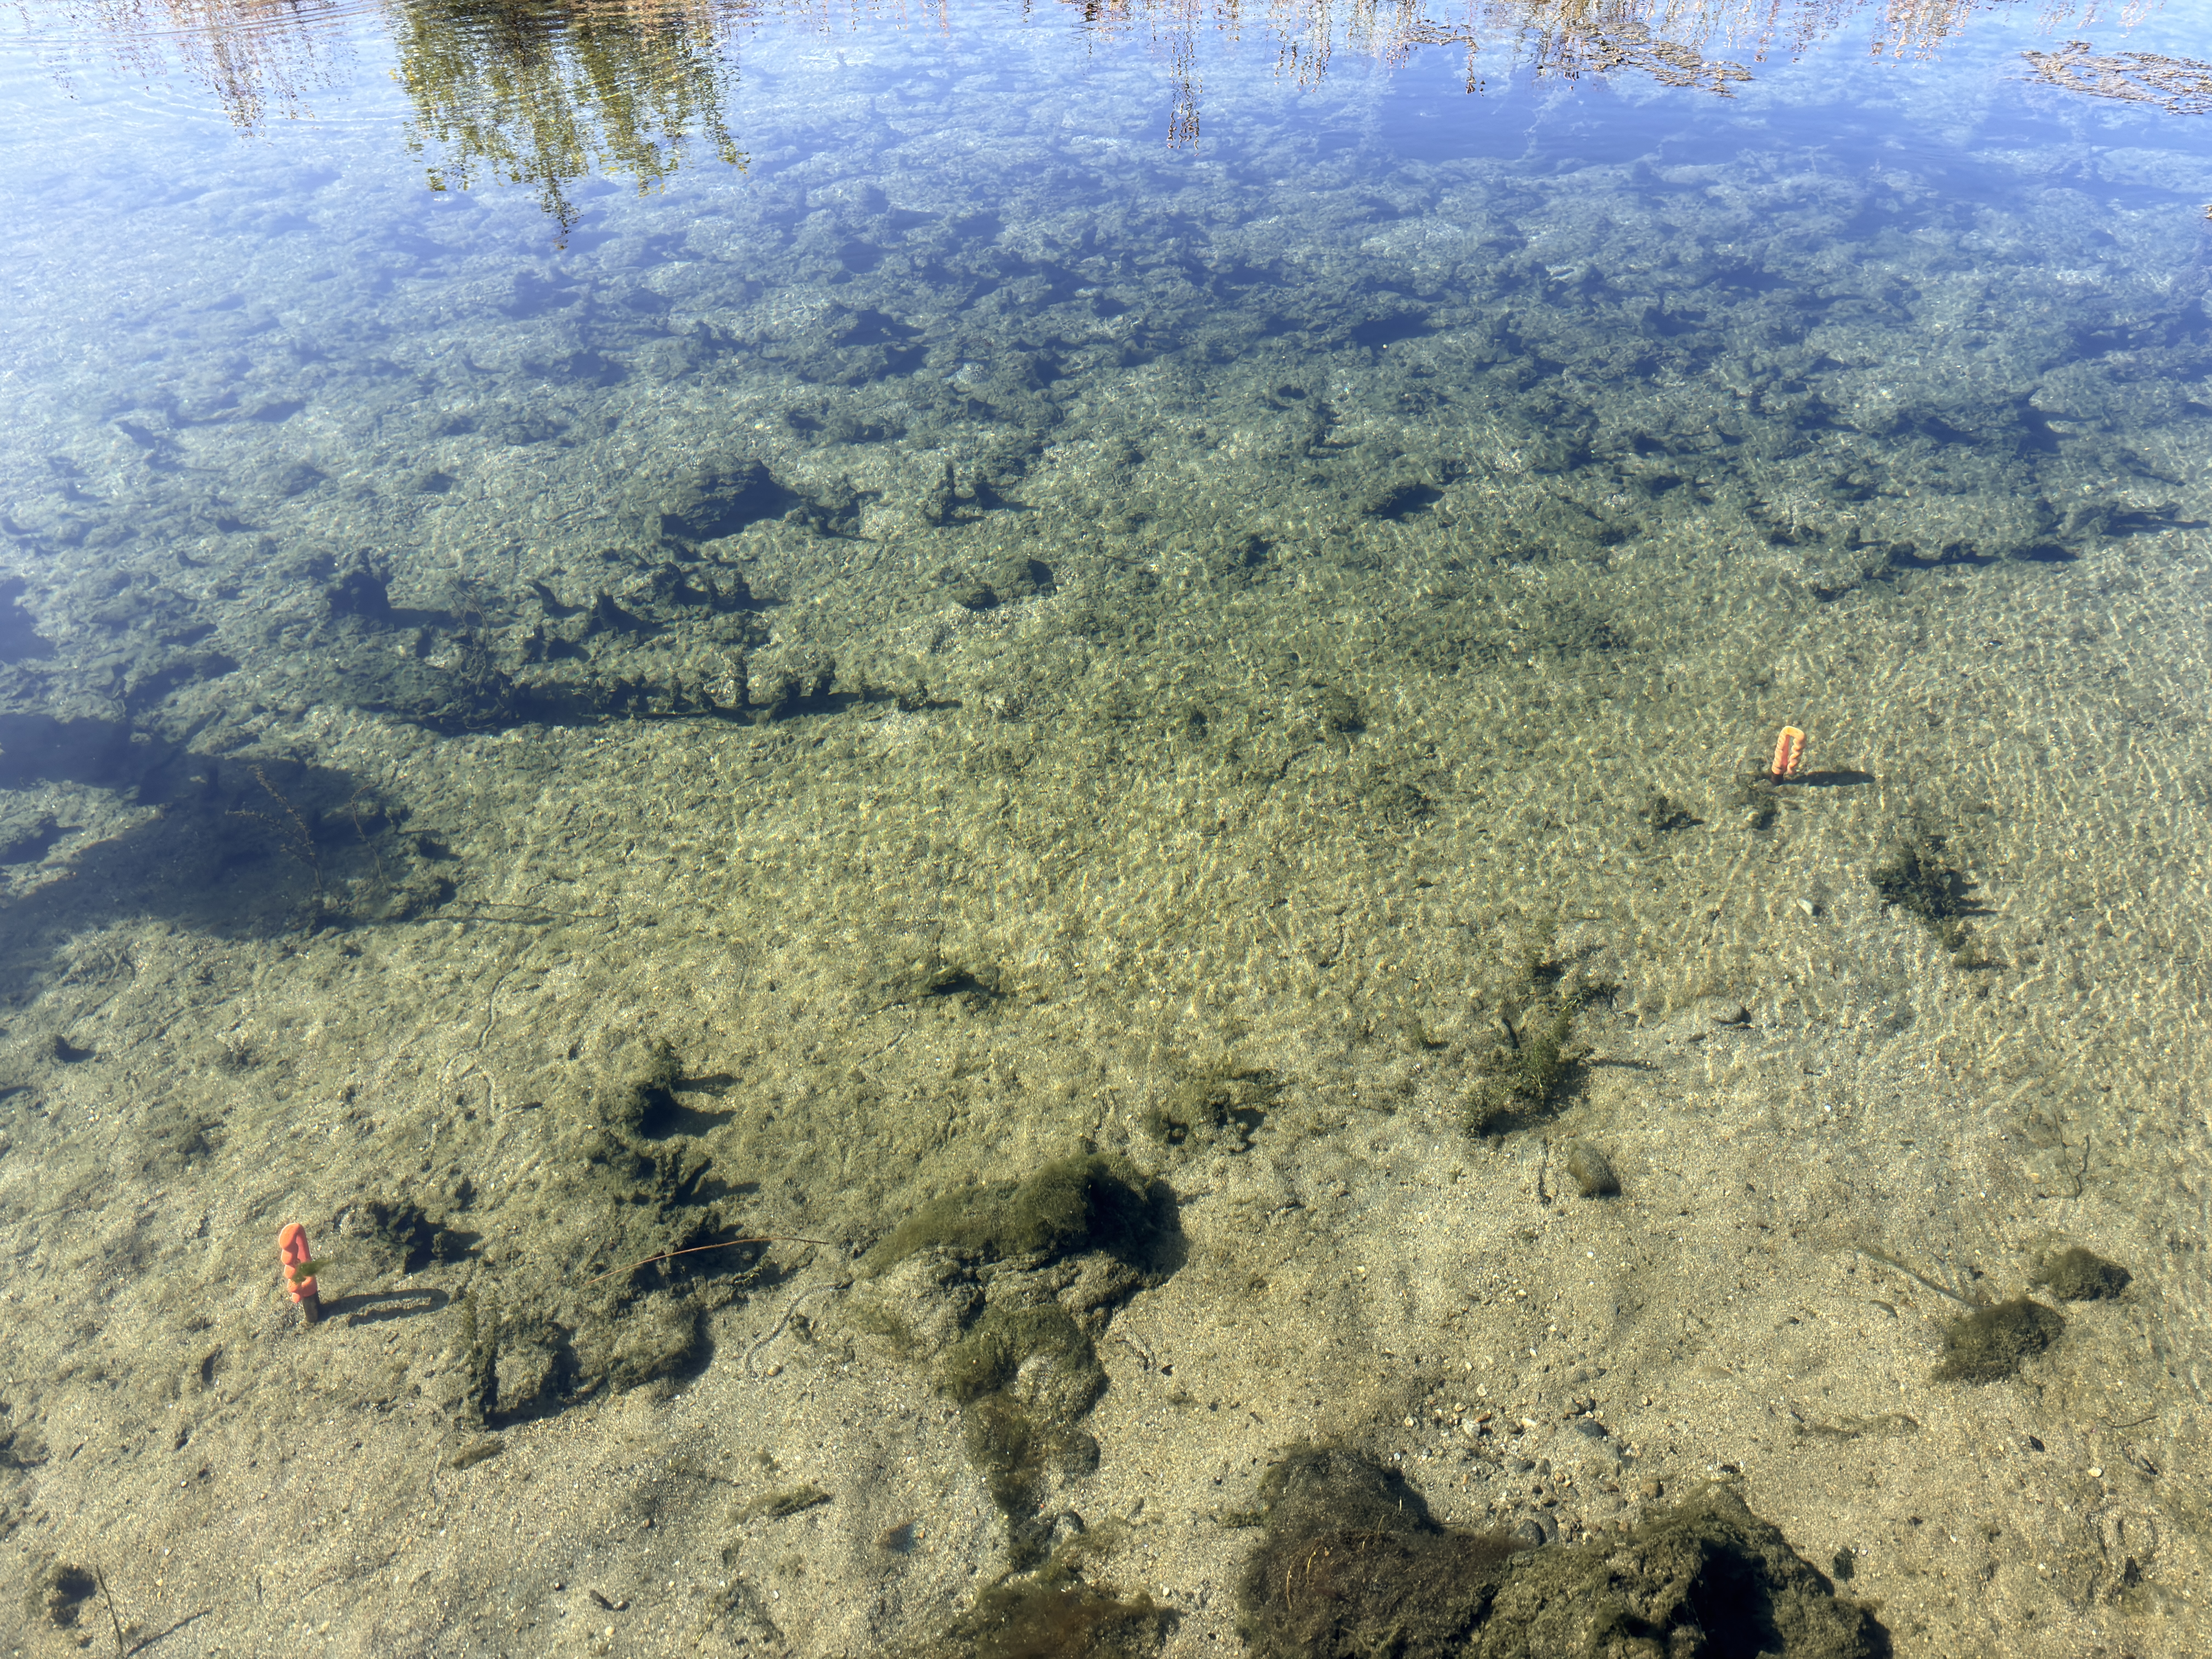
\includegraphics[height=8cm, keepaspectratio]{figure/60_data/area1_riverbed-and-mark.JPG}
    \caption{Area1における検証ターゲットの設置例}
    \label{fig:area1_mark}
  \end{minipage}
  % \hspace{0.5cm}
  \hfill
  \begin{minipage}[t]{0.45\linewidth}
    \centering
    \includegraphics[height=8cm, keepaspectratio]{figure/60_data/area1_mark_measure.jpg}
    \caption{検証ターゲットの測定方法}
    \label{fig:area1_mark_measure}
  \end{minipage}

  % \begin{minipage}[t]{0.45\linewidth}
  %   \centering
  %   \includegraphics[height=5cm, keepaspectratio]{figure/60_data/area1_mark_measure.jpg}
  %   \caption{Area1における検証ターゲット(Point1, Point2)の地点}
  %   \label{fig:area1_mark_measure}
  % \end{minipage}

  % \caption{#8}
  % \label{#9}
\end{figure}

\note{
  Future Work
  撮影時のシャッタースピードは固定できておらず、シャッタースピードに応じたガンマ補正を考慮した輝度値補正を行うべき。
}


% \note{
%   * 偏光レンズを用いたぞ。(これはPlatformに入れるべき話かもしれぬ。)cite(Joyce2018Drone-marine-surveyand_how-to)で、偏光レンズの言及あり(ただし曇りの日)
%   Radiometic Correctionに影響を与えるかもしれないが、どのみち環境光の水面での反射は考慮できていないから、撮影時の河床を鮮明に撮像できることを優先した。
%   * Nadirとオブリークで撮影したぞ。https://gemini.google.com/app/42efe917f2e9b646
%   * 検証点を自分で中に入り、設置し、手動で深度を測定したぞ。それぞれの深度は図のように61cm70cmだったぞ。
%   * 後のWorkflowで解説するが、cite(Joyce2018Drone-marine-surveyandhow-to)によると、水中でのGCP設置は困難であり、SfMによるカメラキャリブレーションの正確性を担保するため、地上を画像内に移せるようにする。
% }

% \note{
%   シャッタースピードが固定されておらず、
%   DJI20251115092203-0002_V.JPG では、1/250で画像が明るくいい感じなのに、
%   DJI20251115092309-0078_V.JPG では、1/640で画像がかなり全体的に暗くなっている。
%   ISPRS前に補正できないか。良くない。
%   https://gemini.google.com/app/42efe917f2e9b646
% }
